\documentclass{article}
\usepackage{longtable}
\usepackage{graphicx}
\usepackage{url}
\usepackage[utf8]{inputenc}
\usepackage{enumerate}
 
\renewcommand{\labelitemi}{$\Box$}
\renewcommand{\labelitemi}{$\star$}
\renewcommand{\labelenumi}{\theenumi}

\usepackage{enumitem,amssymb}
\newlist{todolist}{itemize}{2}
\setlist[todolist]{label=$\square$}

\usepackage{geometry}
 \geometry{
 a4paper,
 total={170mm,257mm},
 left=10mm,
 top=10mm,
 }

\title{Software Quality Assurance Testing MAD5234 2020F}
\author{Peter Sigurdson}
\date{September 2020}

\begin{document}

\maketitle
\includegraphics[scale=.5]{img/MarsClimateOrbiter.png}
\url{https://t2m.io/MAD5234CourseVisualRoadmap}
\section * {Evaluation Schedule}

\begin{itemize}
    \item     Sept 22 Test  1  20\% 
    \item     Sept 30 Test  2 20\% 
    \item     Sept 21 Assignment 1  15\%
    \item     Sept 28 Assignment 2 15\%   
    \item     Sept 15 Activity 1  6\%
    \item     Sept 18 Activity 2  6\%    
    \item     Sept 22 Activity 3  6\%
    \item     Sept 25 Activity 4  6\%     
    \item     Sept 29 Activity 5  6\%
    
\end{itemize}
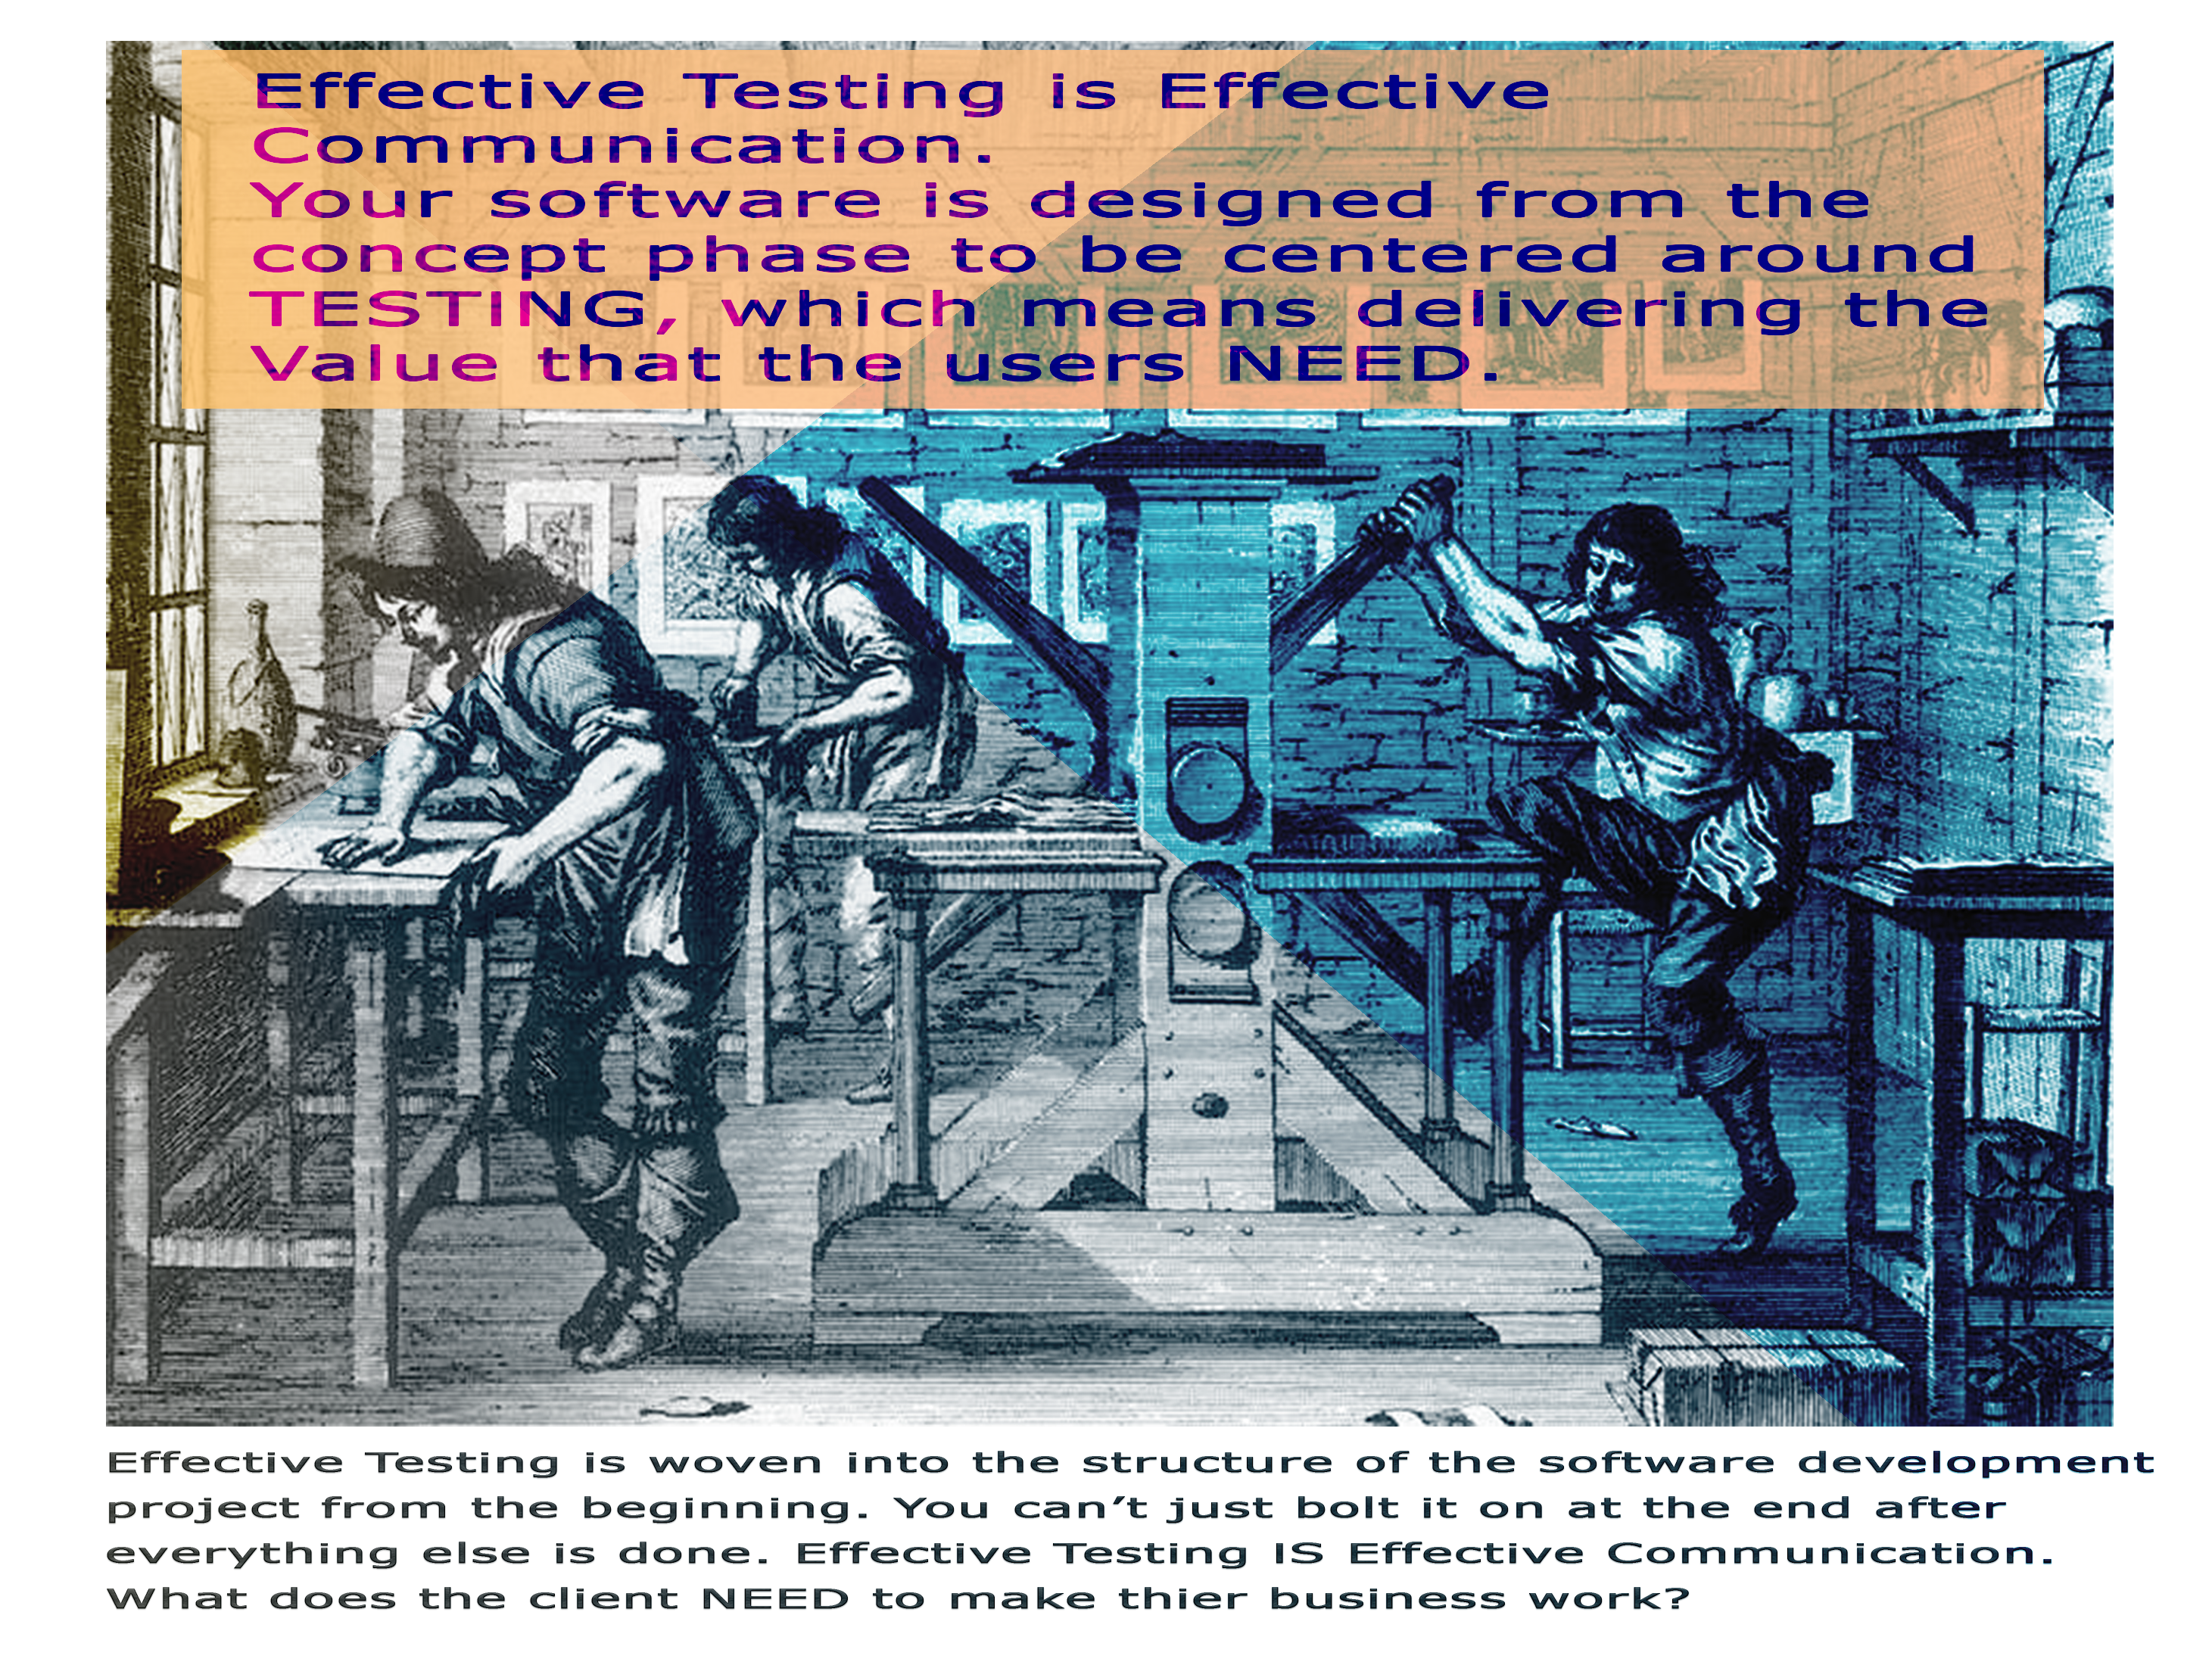
\includegraphics[scale=0.2]{img/softwaretesting.png}

\newpage

\section * {Introduction}
 This course is an introduction to the principles of software quality assurance. \\
 The course addresses the concepts and practices of a software quality assurance function, as well as those aspects of:
 \begin{itemize}
     \item  project management, 
     \item  software design,      
     \item  and testing and configuration management,     
 \end{itemize}
 as applicable to the development of quality software products.
 \newline
 
 \section * {Practices of Software Quality Assurance}   
 \begin{itemize}
     \item Project Management for Software Quality Assurance
     \item Software Design     
     \item Testing and Configuration Management     
 \end{itemize}

Composing bugs may seem like a simple thing. You find a bug, you report it. A lot of people don't consider, good bugs aren't simply a question of the text in the report. There is an inherent structure behind the creation and design of bugs. When delivering feedback, you are not only authoring an issue. You are working within the mindset of your audience, Bug authoring isn't simply about creating issues. It's about documenting the problem. Creating issues paints a picture of what happened, why it happened, and provides some insight on how it may impact the product. It's a process that you work through, whenever you discover something wrong. You will repeat this process continuously, as you discover new issues, and ask yourself a series of questions to ensure you're providing everything the team needs to evaluate and fix the problem. It's central to any bug evaluation to work through all these steps before you start to write up the problem, or it may just end up back in your hands as either incomplete or ignored. First, what happened? What are the details of the issue? You are going to consider the situation closely and spend a lot of time on the details. Remember, people are going to need to understand every nuance and the steps to reproduce the bug. If you click an icon and something crashes, you may want to understand everything you did up to that point when you clicked that icon. It may seem excessive, but it's necessary. When you start to look over an issue, you need to also think about the why of the issue. This is about the mechanics of the bug. This may be immediately obvious in some cases, and in other instances, it could be hidden in the code. While it's not your job to necessarily discover the reason a bug happens, if you can, that's helpful. Knowing why issues happen provides extra value to the developers and speeds the process of addressing the problem. Obviously, you will also want to clearly share where the issue happened with the product. Identify the specific part of the software where an issue occurred. This could be simple on something like a mobile app, but with complicated applications, you may need to provide detailed steps to locate the section of the product that has the issue. Sometimes functions can exist in multiple spaces across a product, and sharing the specific location where the problem exhibited itself can differentiate the source of a bug. One of the core composition requirements is reproducing issues. The problem here is that while some bugs are easy to repeat, some are anomalies, requiring a lot of special circumstances to exhibit themselves. You may experience one-offs that only happened because of a strange and unique series of coincidences. Regardless, it's the duty of any tester to pay close attention to the steps that generated the bug and give the developer a chance to experience it. You may also consider how an issue might be related to other bugs reported up to this point. Each bug can be unique, but it's just as likely that the bug is related to some other problem with the software. Keeping this in mind is critical for bug reporting. Developers don't look at problems the same way testers examine the issues. They are always thinking about the whole product. And good testers also consider this with every discovery. Speaking of unique, every bug should be a single issue or problem. Bugs should never be grouped issues or cover multiple problems. Each submission needs to be a singularly distinctive and reproducible problem. This can get tedious with things like spelling errors, where you document each mistake. However, if they are grouped together, it's possible for the developer to overlook or miss a fix. In our Explore California application, there are APIs, databases and different parts of the user interface, all interrelated and connected. If a bug exhibits itself in one part of the search, it could be related to a lot of different factors. Knowing the issues prior to entering any new discovery helps our team connect the dots when seemingly unrelated issues appear. Those connections are invaluable to the team when they're debugging the reports. Bug composition is a skillset that is developed over time. Some people have a natural ability to report good bugs, while others require training. It's important to take the time to set the ground rules surrounding what your team is looking for in their bugs. Your developers may have specific requirements to help them debug problems. Taking the early steps to discover the needs of your development partners will help keep your discoveries important and relevant.
\section *  {Course Learning Outcomes/Course Objectives}
\begin{itemize}

     \item     1. Evaluate software testing and quality assurance techniques as part of an integrated discipline of software quality verification and validation.

     \item      1.1 Discuss the discipline of software engineering  
     \item      1.2 Discuss the importance of software quality attributes.
     \item      1.3 Analyze the software testing lifecycle.
     \item      2. Assess software foundations, program correctness and verification and various failures, errors and faults and methods of software testing taxonomy.
     \item      2.1 Discuss the foundations of proper software properties, specifications and reliability versus safety.
     \item      2.2 Analyze and compare examples of program verification and correctness.
     \item       2.3 Evaluate and determine courses of action taken from examples of failures, errors and faults.
      \item      2.4 Analyze methods related to software testing taxonomy.
     \item      3. Evaluate test generation concepts using functional and structural criteria.
     \item      3.1 Discuss test generation concepts.
     \item      3.2 Analyze examples of functional criteria.
     \item      3.3 Analyze examples of structural criteria.
     \item      4. Evaluate specifications of drivers and industry standards such as Oracle.      
     \item      4.1 Test oracle design specifications.     
     \item      4.2 Test driver design specifications.       
     \item      4.3 Test outcome analysis             
     \item      5. Discuss and evaluate the management of software testing.          
     \item      5.1 Discuss and analyze examples of metrics for software testing.          
     \item      5.2 Use software testing tools.  
     \item      5.3 Analyze and test product lines.     

     
 \end{itemize}

     


\newpage
\section * {Teaching Day Plan}

\begin{longtable}{ l  }
 \hline
    \\
    Day 01 MON Sept 14 \\ \\ 
     1. Evaluate software testing and quality assurance techniques as part of an integrated discipline of software quality verification and validation.\\
            1.1 Discuss the discipline of software engineering.\\
            1.2 Discuss the importance of software quality attributes.\\
            1.3 Analyze the software testing life-cycle.\\ \\
    \hline 
    \\         
    Day 02 TUE Sept 15 \\  \\ 
            2.1 Discuss the foundations of proper software properties, specifications and reliability versus safety. \\
            2.2 Analyze and compare examples of program verification and correctness. \\
		    Activity 1  6\% \\   \\   
    \hline 
    \\    Day 03 WED Sept 16 \\ \\ 
          2.3 Evaluate and determine courses of action taken from examples of failures, errors and faults. \\ \\ 
     \hline   
     \\       Day 04 THU Sept 17 \\    \\ 
        Review and reinforcement of topics covered so far: In class Review Activity \\
           2.4 Analyze methods related to software testing taxonomy. \\  \\ 
     \hline    
     \\        Day 05 FRI Sept 18 \\ \\ 
           3.1 Discuss test generation concepts. \\
             Activity 2  6\% \\ \\ 
      \newpage 
      \hline   
      
    \\          Day 06 MON Sept 21 \\ \\ 
            3.2 Analyze examples of functional criteria. \\
            Assignment 1  15\% \\ \\ 
      \hline   
     \\        Day 07 TUE Sept 22 \\ \\ 
         3.3 Analyze examples of structural criteria. \\
            Activity 3  6\% \\
           Test  1  20\%  \\ \\ 
      \hline   
    \\          Day 08 WED Sept 23 \\ \\ 
            4.1 Test oracle design specifications. \\
            4.2 Test driver design specifications. \\ \\ 
       \hline  
    \\         Day 09 THU Sept 24 \\ \\ 
            4.3 Test outcome analysis. \\ \\ 
       \hline  
    \\          Day 10 FRI Sept 25 \\ \\ 
            5.1 Discuss and anlayze examples of metrics for software testing. \\
            Activity 4  6\% \\ \\ 
      \hline   
    
    \\          Day 11 MON Sept 28 \\ \\ 
            5.2 Use software testing tools. \\
            Assignment 2 15\% \\ \\ 
      \hline   
    \\          Day 12 TUE Sept 29 \\ \\ 
            5.3 Analyze and test product lines. \\
            Activity 5  6\% \\ \\ 
    \hline     
    \\          Day 13 WED Sept 30 \\ \\ 
            Review and Reinforce All Topics \\
            Test  2 20\%  \\ \\ 
      
\end{longtable}
\newpage

\end{document}
